\chapter{Methodology}
This chapter details the methods used in this dissertation. Specifically, the focus is on collaborative genre tagging (CGT) - a two-step approach that applies collaborative filtering to predict genres of items such as movies or books. First, CGT is outlined and compared to more common uses of collaborative filtering on data sets such as MovieLens and Goodbooks. Then, the model architecture of CGT is detailed, along with the key hyperparameters to be tuned. Finally, the framework for hyperparameter tuning and model evaluation is described with special attention given to the reproducibility of results.

\section{Collaborative genre tagging}
Most of the previous work on collaborative filtering (CF) tackled the problem of predicting user preferences using their interaction history. The most successful methods all involve the use of latent factor models which are capable of learning otherwise hidden properties in the users and items in CF datasets. Recently this type of approach has been adapted from matrix factorisation models to neural architectures which capture latent factors in embedding layers, while allowing for non-linearity in successive hidden layers. 

CF models, by definition, do not make use of meta data for predicting user preferences -- this is the domain of content-based models. However, meta data such as item genres are still useful to users for assessing recommendations provided to them. Users cannot be expected to trust recommendations provided to them, without having some sort of description of the recommended item. While CF has shown its ability to provide recommendations to users without using content attributes, descriptive features are still useful for users to make informed decisions on \textit{which} recommendations to choose.

In this Master's dissertation, a new application of CF for predicting item genres from explicit user ratings is explored, dubbed collaborative genre tagging, or CGT. This method uses a two-headed architecture which shares a common embedding layer. The first head of the model is used to train the embedding layer, while the second head is used to learn how to predict item genres from trained embedding weights. Figure \ref{fig:4_CGT-architecture} shows the connected architecture of the CGT model.

\begin{figure}[H]
\centering
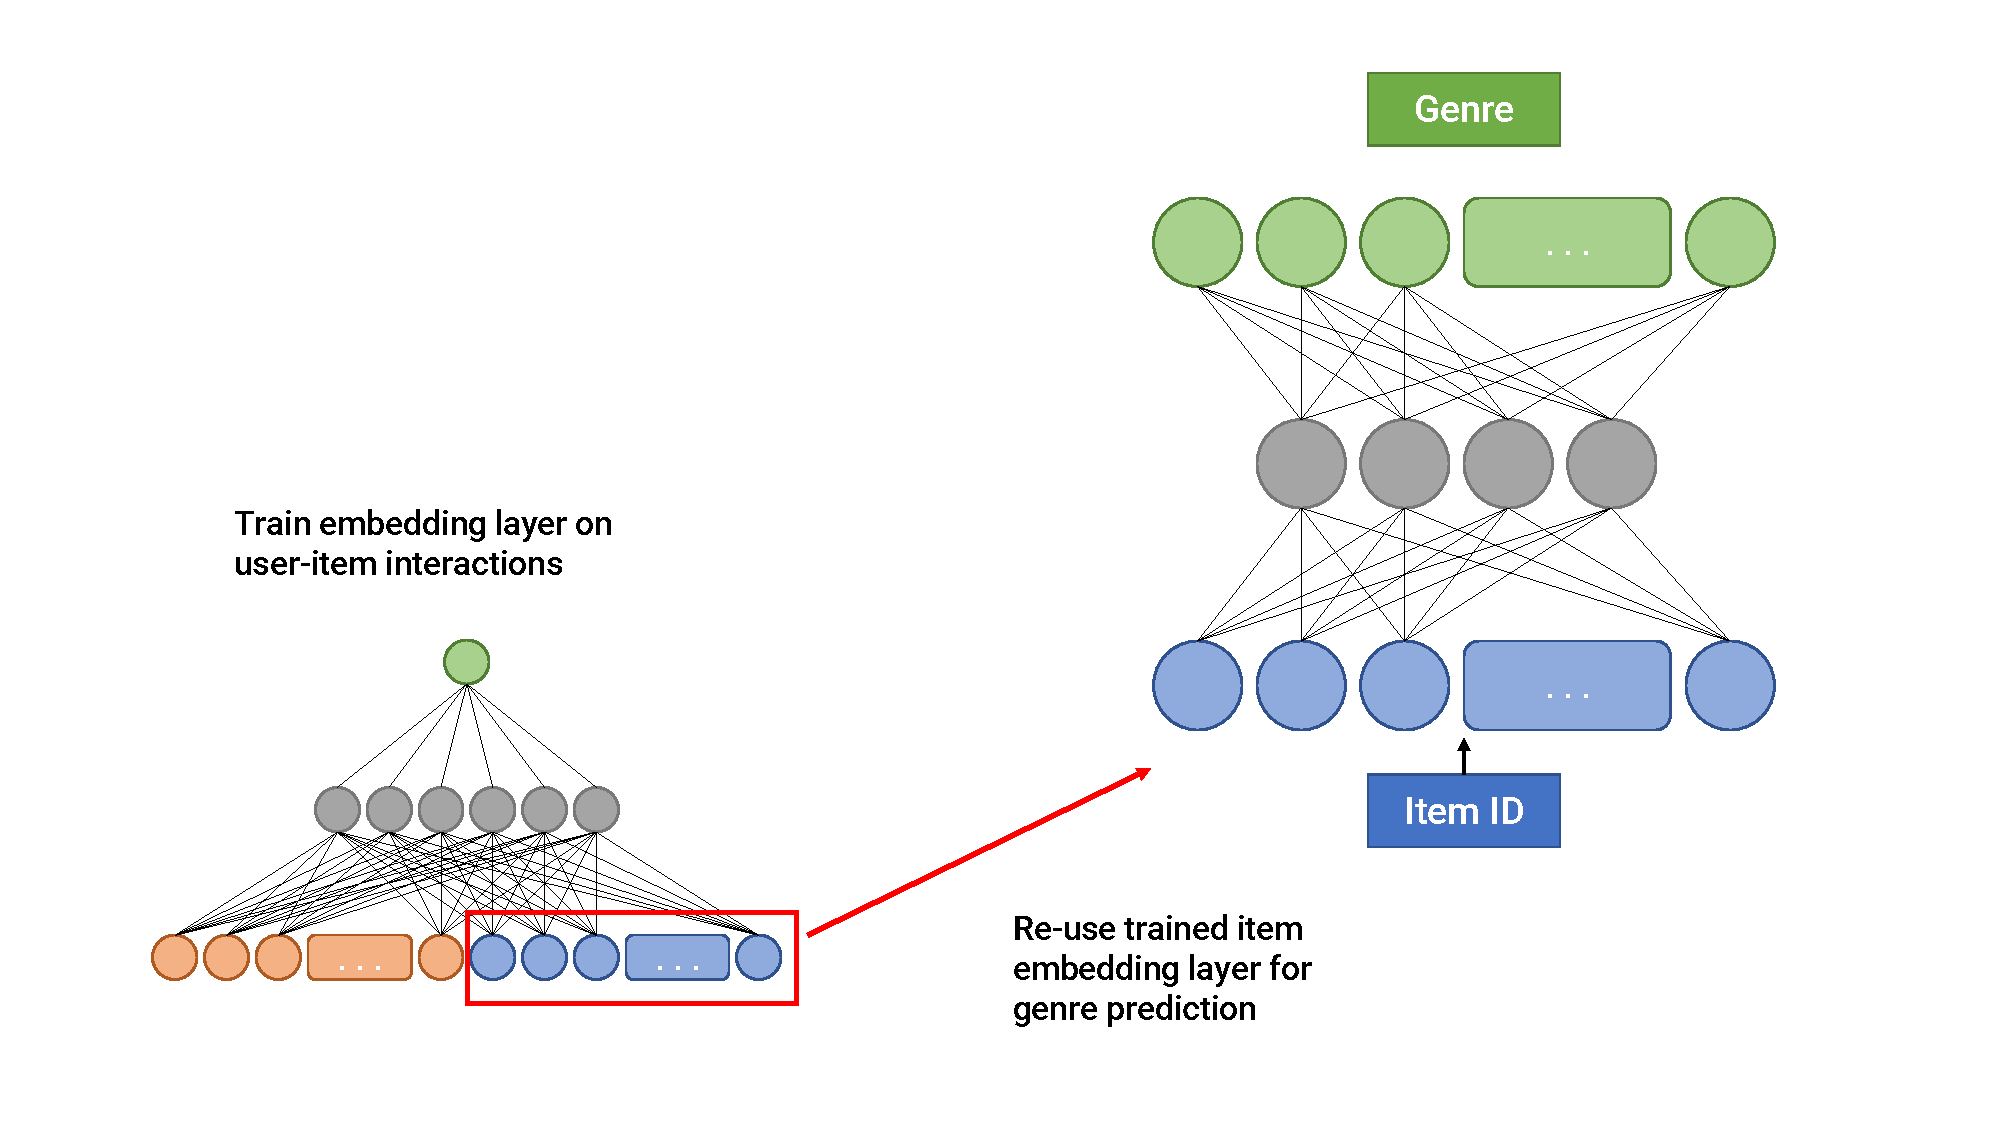
\includegraphics[width=0.95\textwidth]{Figures/4_CGT-model.pdf}
\decoRule
\caption[CGT architecture]{CGT model consists of two neural networks which share a common item embedding layer}
\label{fig:4_CGT-architecture}
\end{figure}

The first head of the CGT model uses latent factors to predict user ratings and is similar in construct to the Neural Collaborative Filtering model used by \citeauthor{he2017neural} (the architecture of which is shown in figure \ref{fig:ncf-arch}). The purpose of this model is to train the embedding layer to produce latent factors associated with every item in the ratings dataset.

After training the first head of the CGT model, the trained item embedding layer is then frozen and used as the first layer of the second head. The second head then learns a mapping from item embedding to item genre.

\section{Rating model}
The rating model is the base of the CGT model. The input to this model is a user-item ID pair, and the output is an explicit rating. The IDs in the input pair are connected to an embedding layer of $k\times2$ length, where $k$ is the number of latent factors for both users and items. The embedding layer then feeds to a fully connected layer and then finally into a single output node which contains the predicted rating.

\begin{figure}[H]
\centering
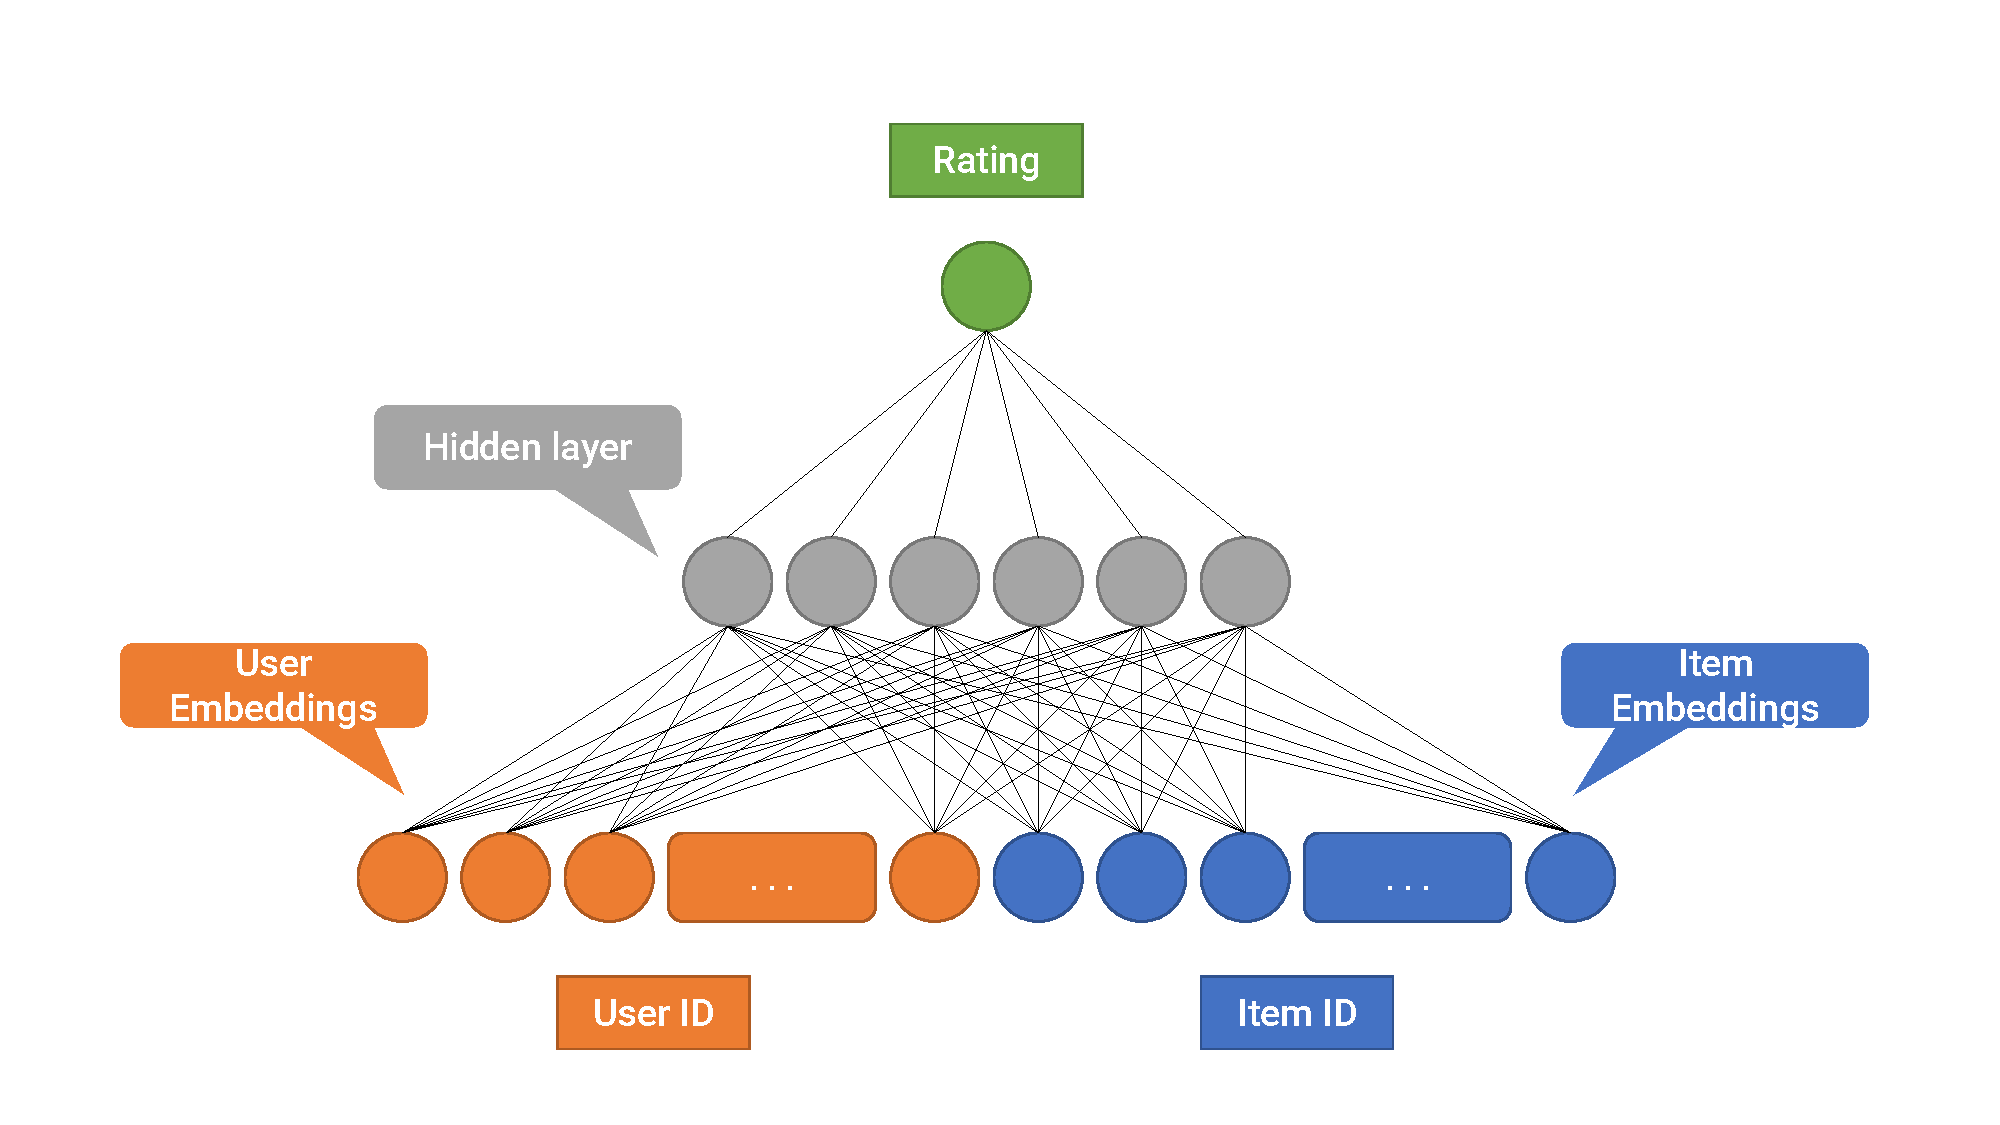
\includegraphics[width=0.95\textwidth]{Figures/4_ratings-model.pdf}
\decoRule
\caption[Rating model]{Rating model uses embeddings to capture latent factors of items and users}
\label{fig:4_rating-prediction-architecture}
\end{figure}

\subsection{Embedding layer}
The first layer of the rating model is a concatenated embedding layer. This layer is comprised of two separate embedding matrices, the same as those used in the matrix factorisation method popularised by \citeauthor{koren2009matrix}. These embedding matrices hold the latent factors of all users and items respectively. The user matrix is of dimension $m\times k$ while the item matrix is $n\times k$, where $m$ and $n$ are the number of distinct users and items respectively, and $k$ is the number of latent factors. $k$ is a hyperparameter which will need to be tuned.

\begin{figure}[H]
\centering
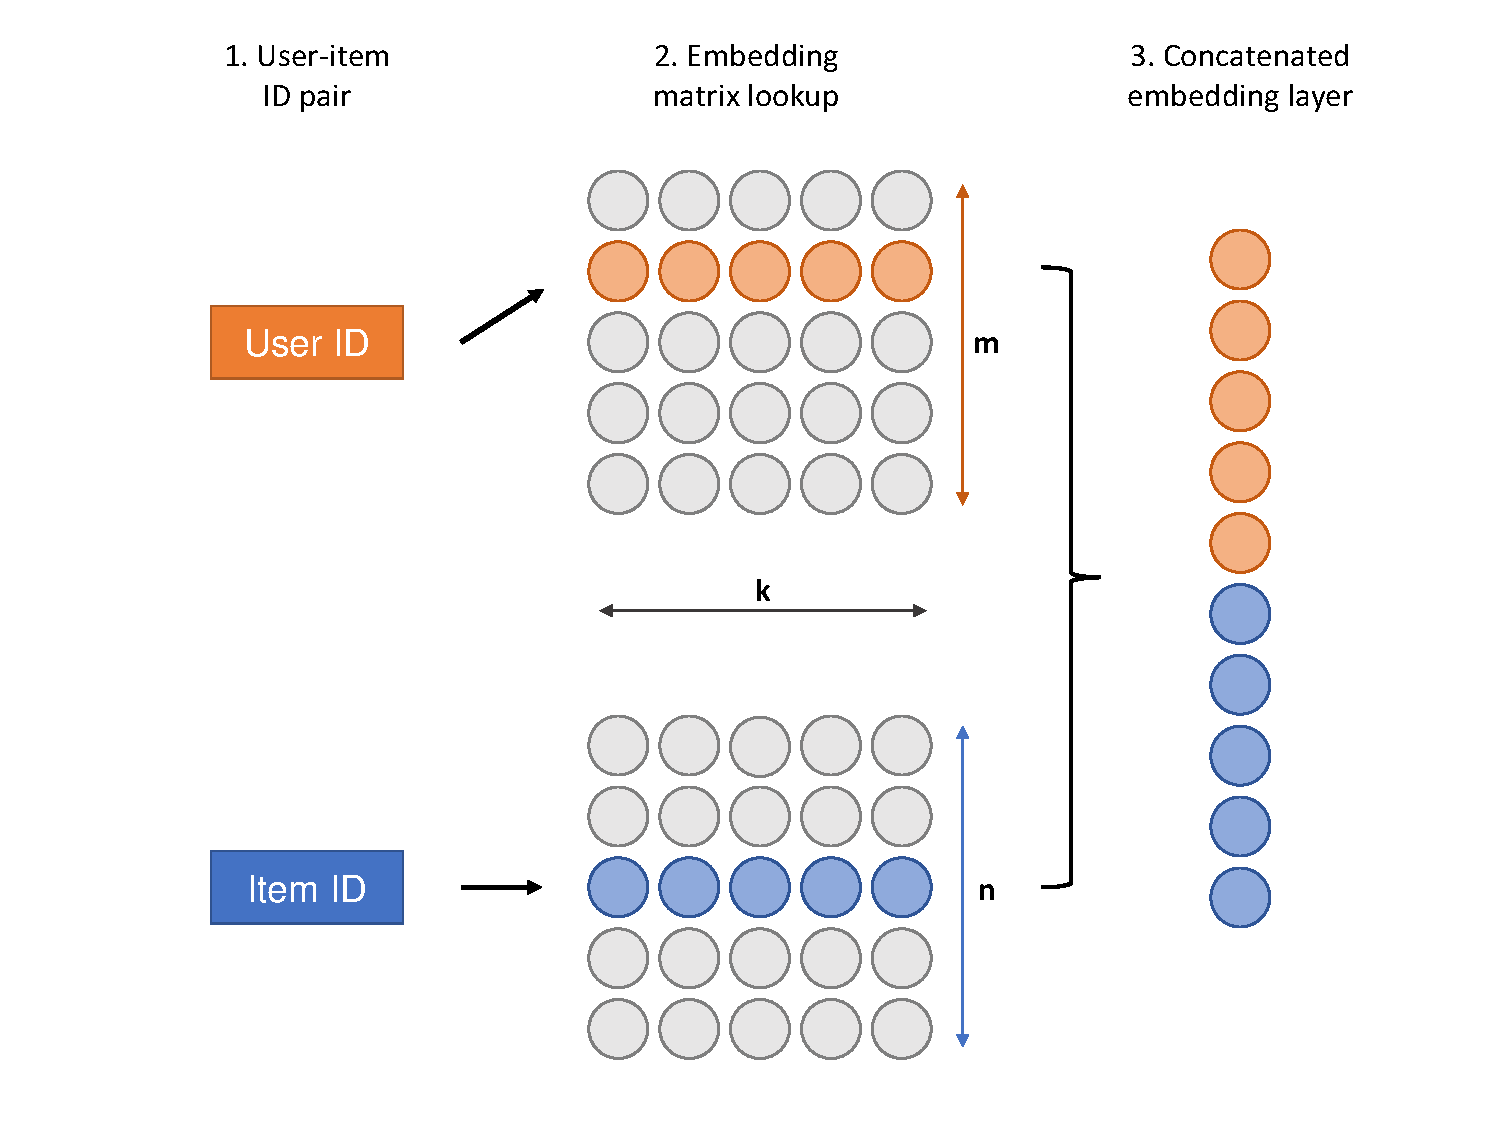
\includegraphics[width=0.85\textwidth]{Figures/4_CGT-embedding-layer.pdf}
\decoRule
\caption[Embedding layer]{Embedding layer is created as the concatenation of two separate embedding matrix lookups.}
\label{fig:4_CGT-embedding-layer}
\end{figure}

\subsection{Hidden layer}
Talk about number of neurons, activation function and dropout rate.

\subsection{Output layer}
\begin{figure}[H]
\centering
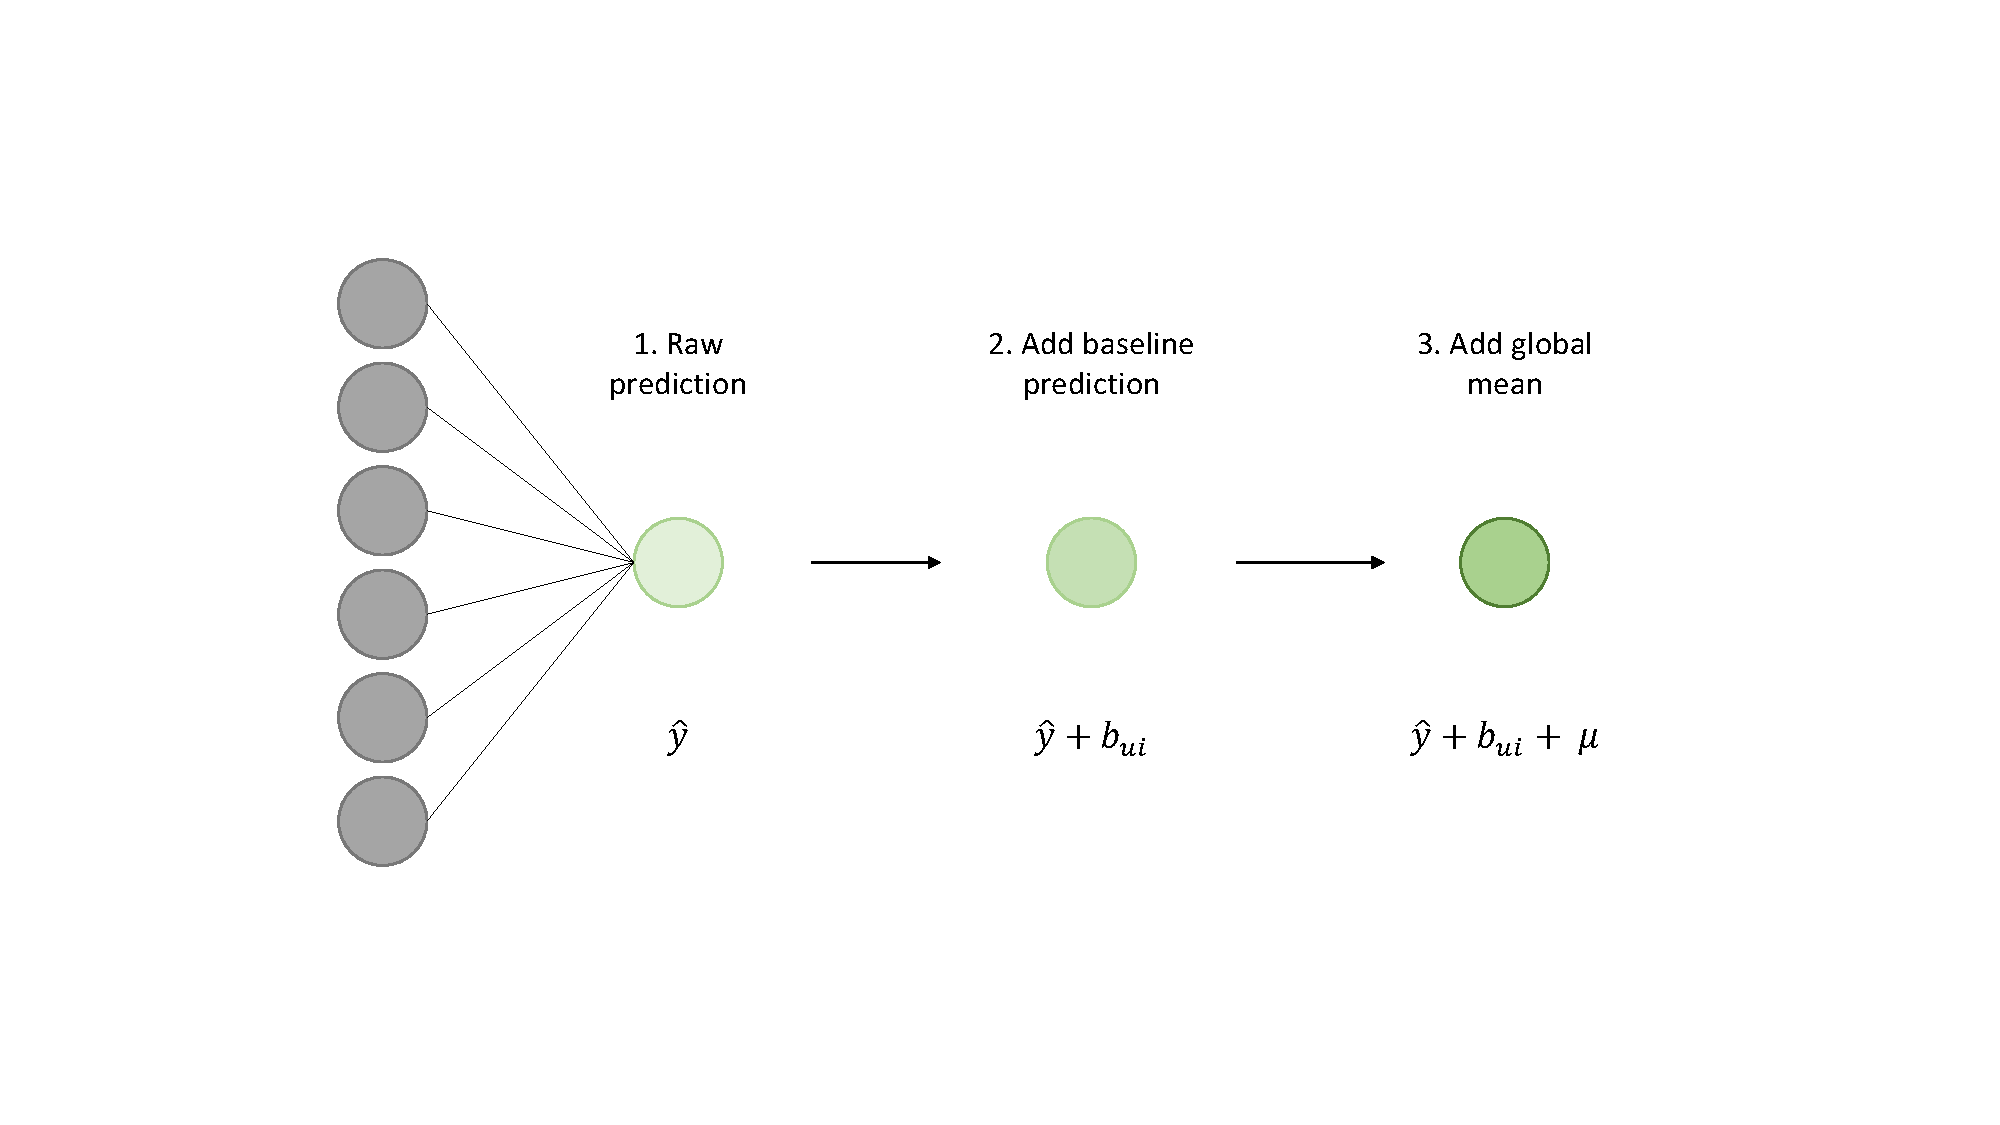
\includegraphics[width=0.9\textwidth]{Figures/4_CGT-output-layer.pdf}
\decoRule
\caption[Rating layer]{Model output is adjusted through the addition of baseline predictors.}
\label{fig:4_CGT-rating-layer}
\end{figure}

\textbf{add some equations here}

\subsection{Hyper parameters}

\section{Genre prediction}

\subsection{Model architecture}
\begin{figure}[H]
\centering
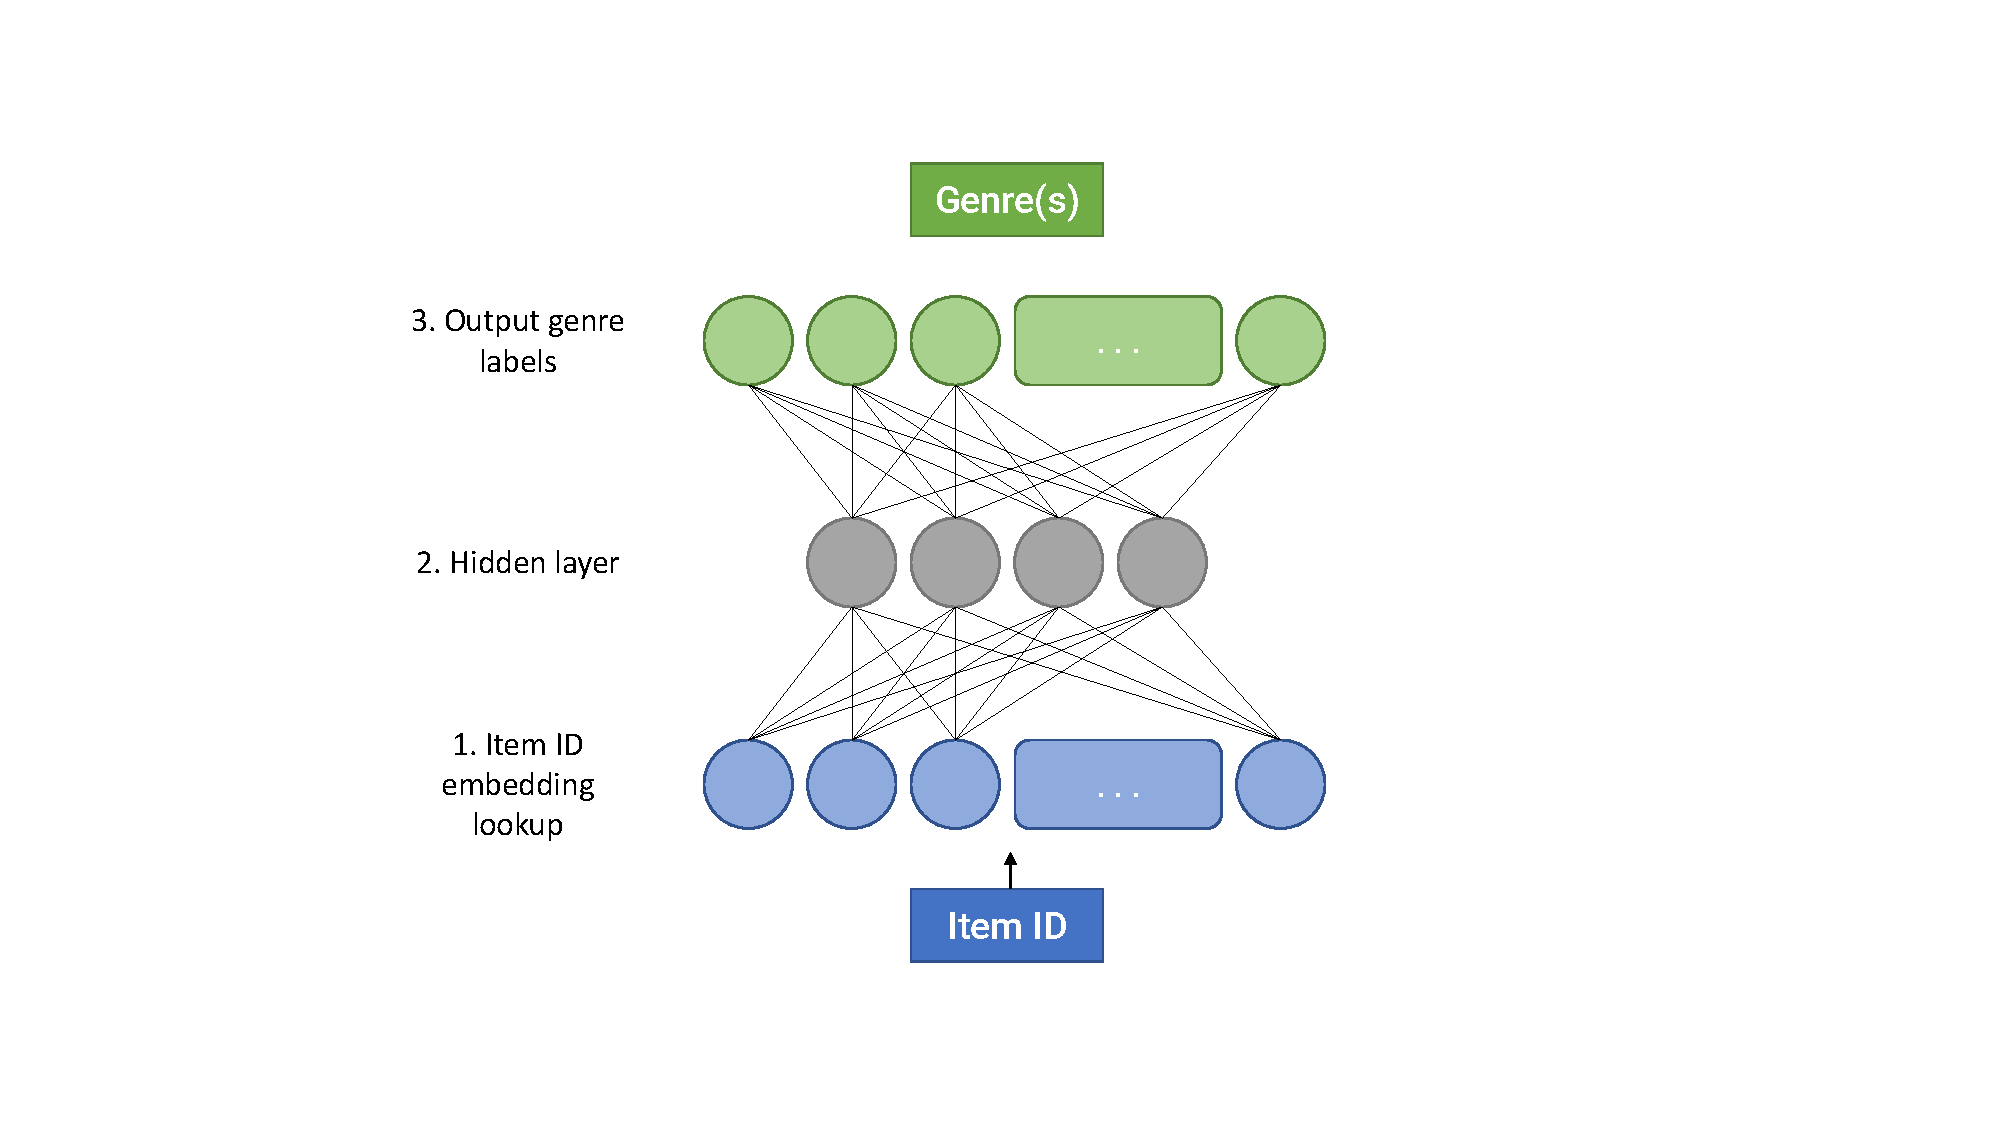
\includegraphics[width=0.9\textwidth]{Figures/4_genre-model.pdf}
\decoRule
\caption[Genre prediction model]{Genre prediction model re-uses the item embedding layer from the base ratings prediction model}
\label{fig:4_genre-prediction-architecture}
\end{figure}

\subsection{Hyper parameters}